\documentclass[nocopyrightspace]{sigplanconf}
\usepackage{amsmath}
\usepackage{graphicx}
\usepackage{multirow}
\usepackage[english]{babel}
\usepackage{tabularx}
\usepackage{booktabs}


\title{Machine Learning Model for Detecting \\Code Clone Related Bugs}

\authorinfo{Chowdhury Ashabul Yeameen}
           {The University of Texas, Dallas}
           {cxy111130@utdallas.edu}
           
\authorinfo{Seungtak Baek}
		   {The University of Texas, Dallas}
		   {sxb085000@utdallas.edu}

\date{}

\begin{document}

\maketitle

\begin{abstract}
Studies found that many large software contain significant clone codes. Though intentional copy-paste activities can be considered as the replication of tested code, they can also lead to a difficult to maintain codebase because there are multiple places to update for single modification. Failed to update all the places, which is quite common in duplicate code due to various reasons, results in inconsistent clones. Sometimes asymmetric modifications happen just because that part needed some added/modified functionality. But many other times those changes are intended to fix a bug in it. And since the link between clones are usually not maintained, that modification does not propagates and that particular bug remains alive on its clone(s).

\vspace{10 pt}
\noindent
Detecting clone related bugs due to inconsistent change has gained research interest among the researchers in recent time. All of these heuristic based approaches show some success in detecting clone related bugs but still suffers from low accuracy of 10\%-30\%. We have created a machine learning model which use the clone copies from a any clone related bug detection method, learn the signs of bugs from the differences in near match clones, and improve accuracy significantly over the source method. We considered several different techniques to extract features and tried with multiple machine learning algorithms to show their relative performance on our dataset. Lastly we have interpreted the significance of precision and recall our model achieved in detecting harmful code in a software.
\end{abstract}
			
\section{Introduction}
Intentional code cloning, otherwise known as copy-paste of codes, is considered as a bad practice in Software Engineering. But sometimes there are no alternatives other than cloning when some code is used as a template or sequence of function call is necessary for achieving some functionality. Example of these cases are hardware drivers where people use some kind of template to start with and resource allocation/deallocation methods which are used sequentially and repeated over and over in many places in a software code. Some recent studies found its unavoidable as clone code exist in all major large scale software~\cite{Li2006,Kamiya2002,Baker1995}. The study by \emph{Kamiya et al}~\cite{Kamiya2002} found that 12 percent of Linux code was actually duplicate whereas \emph{Baker}~\cite{Baker1995} showed 19 percent of X Window System showed the sign of duplications.

\vspace{10 pt}
\noindent
\emph{Juergens et al}~\cite{Juergens2009} presented how do inconsistent code clones affect software quality, by answering their research question “can inconsistent clones be indicators for faults in real systems?” The researchers analyzed 4 commercial projects and 1 open sources project. As a result, they found 3-23\% of the inconsistent clones being actual faults. To this research question, they concluded that inconsistent code clones had statistically more faults than the average code, thus “inconsistencies can be indicators for faults in real systems.” A study of \emph{Code Clone Genealogy}~\cite{Kim2005} showed even active refactoring followed by many agile methodologies is not enough to remove all the clone codes.

\vspace{10 pt}
\noindent
There are many techniques for suggested for detecting exact and near match code clones.\emph{Baker}~\citep{Baker1995} took line-by-line approach. That is, they first abstracted lexical units, such as function identifiers, variable names and types with parameter identifier. Then, using a suffix-tree algorithm, they found matches among this result. Yet, Dup had major problem with line restructuring. Dup could not detect matches even if the only difference between two lines was a line break. 

\vspace{10 pt}
\noindent
Similar to this approach, \emph{Duploc}~\cite{Ducasse1999} overcame the problem above. Using string-based Dynamic Pattern Matching, this tool could detect matches even with gap existing between lines. However, Duploc too had problem: the performance. The complexity of Duploc is $O(n^2)$, whereas that of Dup is only $O(n)$. Ducasse et al alleviated this challenge somewhat through using hash table for string.

\vspace{10 pt}
\noindent
\emph{I. Baxter et al}~\cite{Baxter1998} and \emph{Lingxiao Jiang et al}~\cite{Jiang2007} used Abstract Syntax Tree in effort to extract code clones from C projects. Their tool includes macros in the process of building AST in effort to build more complete AST. In this approach with hash function, one can detect clones with gap and even ones with line reordering. It seems that this approach solves most of the problem. Yet, this approach suffers from heavy computing power, since it requires full syntax analysis.
\begin{figure*}[t!]
\centering
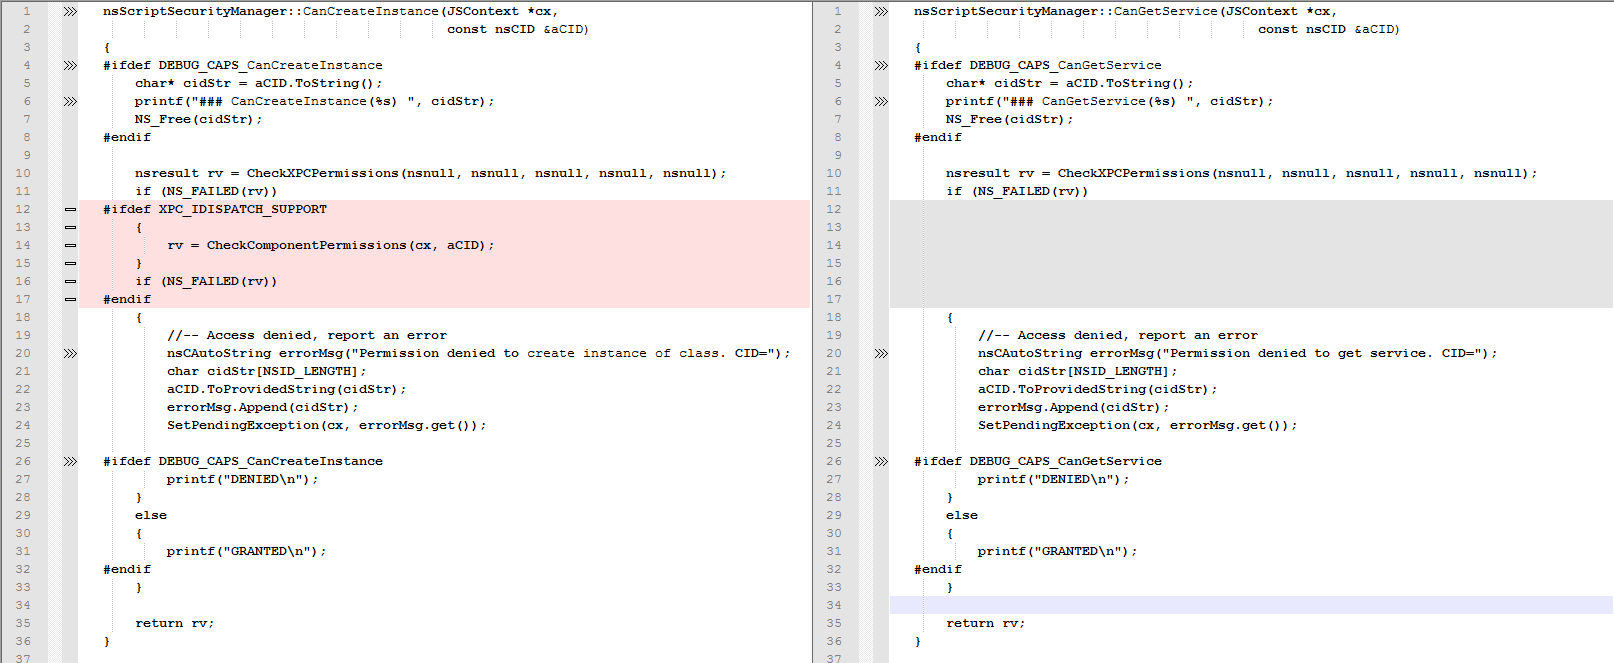
\includegraphics[width=\textwidth]{BugCase.png}
\caption{Near match clone copies with bug fix}
\label{fig:buggy}
\end{figure*}

\begin{figure*}[t!]
\centering
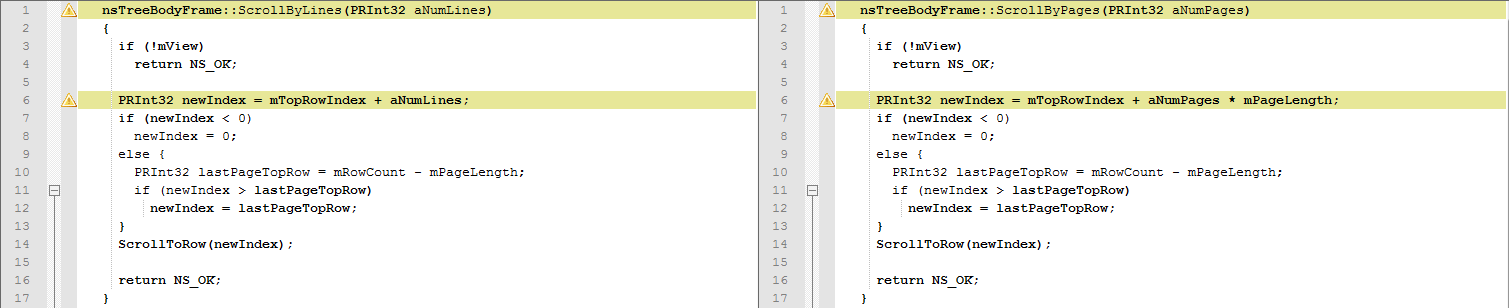
\includegraphics[width=\textwidth]{Benigncase.png}
\caption{Near match clone copies with benign change}
\label{fig:benign}
\end{figure*}

\vspace{10 pt}
\noindent
More coarse grained approach has been attempted. \emph{Mayrand et al}~\cite{Mayrand1996} used function-by-function approach. With this scheme, each function body was to be represented by Intermediate Representation Language (IRL). Then, functions with similar metric values in IRL were paired as clones.Another promising tool is \emph{Similar method Classifier (SMC)}~\cite{Balazinska1999}. This tool incorporates both metric value-based approach and DPM. It will first extract function body and represent each function with metric values. Using the computed metric values, we identify pairs. After we extracted possible clone pairs, we apply token analysis using DPM. The end result of this approach is a list of clones in 18 classes. Even if the paper only applied this approach to whole function body only, this approach can also be applied to part of a function, with minor adjustments.\emph{Zhenmin Li et al}~\citep{Li2006} used frequent subsequence mining of tokens whereas \emph{Kamiya et al}~\cite{Kamiya2002} used sequence of tokens for detecting code clones. 

\vspace{10 pt}
\noindent
There are some recent researches on detecting clone related bugs. But all of these approaches are based on some heuristics and/or rule based techniques. \emph{Deckard}~\cite{Jiang2007} considers difference of contexts in the clones. The study by \emph{Dawson Engler et al}~\cite{Engler2001} goes even further to find anomaly in frequently used template code as a sign of bug and come up with decent accuracy, and more importantly, ranking of possibility of those bugs in OpenBSD code base. \emph{Mark Gabel et al.}~\cite{Gabel2010} proposed a scalable tool \emph{DejaVu}, an independent and extended implementation of \emph{DECKARD} to detect bug in a 75+ million lines of code base and achieved 30 percent accuracy. Though applying many such heuristics and relaxed matching improve recall, all the techniques heavily suffers from accuracy or recall. We took off where other methods left off - get near match clones by using existing techniques, extract features, and apply machine learning techniques to improve accuracy. After applying machine learning technique, accuracy improved more than 2-fold to any existing work with over $80\%$ on the sample case of finding bug in Firefox codebase.

\section{Overview}
\subsection{Task Definition}

\begin{table*}[htb!]
\centering
\begin{tabularx}{\textwidth}{|X|X|X|X|X|X|X|X|X|X|}
\hline
\multicolumn{1}{|c|}{\multirow{2}{*}{Powers}} & 
\multicolumn{1}{|c|}{\multirow{2}{*}{Meta}} & 
\multicolumn{1}{|c|}{\multirow{2}{*}{Parameter}} & 
\multicolumn{3}{|c|}{Harmful} & 
\multicolumn{3}{|c|}{Benign} & 
\multicolumn{1}{|c|}{\multirow{2}{*}{Overall}} \\
\cline{4-9}

& & & Correct & Missed & Recall & Correct & Missed & Recall & \\
\hline

SVM & & G=0.2 & 92 & 4 & 95.8\% & 8 & 26 & 23.5\% & 76.92\% \\
\hline
SVM & AdaBoost & G=.2,I=30 & 83 & 13 & 86.5\% & 17 & 17 & 50\% & 76.92\% \\
\hline
SVM	& Bagging& G=.2,I=30  & 92 & 4 & 95.8\% & 8 & 26 & 23.5\% & 76.92\% \\
\hline
NB & & & 83 & 13 & 86.5\% & 22 & 12 & 64.7\% & 80.77\% \\
\hline
NB & Bagging & I=30 & 85 & 11 & 88.5\% & 21 & 13 & 61.8\% & 81.53\% \\
\hline
\end{tabularx}
\caption{Effectiveness on Recalling Bug, Check and Smell}
\label{tab:dataset1}
\end{table*}

\begin{table*}[htb!]
\centering
\begin{tabularx}{\textwidth}{|X|X|X|X|X|X|X|X|X|X|}
\hline
\multicolumn{1}{|c|}{\multirow{2}{*}{Powers}} & 
\multicolumn{1}{|c|}{\multirow{2}{*}{Meta}} & 
\multicolumn{1}{|c|}{\multirow{2}{*}{Parameter}} & 
\multicolumn{3}{|c|}{Harmful} & 
\multicolumn{3}{|c|}{Benign} & 
\multicolumn{1}{|c|}{\multirow{2}{*}{Overall}} \\
\cline{4-9}

& & & Correct & Missed & Recall & Correct & Missed & Recall & \\
\hline
NB &  &  & 98 & 8 & 92.5\% & 17 & 7 & 70.8\% & 88.46\% \\ 
\hline 
NB & AdaBoost & I=30,P=100 & 98 & 8 & 92.5\% & 16 & 8 & 66.7\% & 87.69\%\\ 
\hline 
NB & AdaBoost & I=30,P=50 & 98 & 8 & 92.5\% & 18 & 6 & 75\% & 89.23\% \\ 
\hline 
SVM &  & G=.2 & 106 & 0 & 100\% & 7 & 17 & 29.2\% & 86.92\%\\ 
\hline 
SVM & AdaBoost & G=.2,I=30 & 100 & 6 & 94.3\% & 15 & 9 & 62.5\% & 88.46\%\\ 
\hline 
SVM & AdaBoost & G=.2,P=50 & 100 & 6 & 94.3\% & 16 & 8 & 66.7\% & 89.23\%\\ 
\hline 
SVM & Bagging & I=10 & 105 & 1 & 99.1\% & 9 & 15 & 37.5\% & 87.7\%\\
\hline
\end{tabularx}
\caption{Effectiveness on Reducing False Cases}
\label{tab:dataset2}
\end{table*}

\begin{table*}[htb!]
\centering
\begin{tabularx}{\textwidth}{|X|X|X|X|X|X|X|X|X|X|}
\hline
\multicolumn{1}{|c|}{\multirow{2}{*}{Powers}} & 
\multicolumn{1}{|c|}{\multirow{2}{*}{Meta}} & 
\multicolumn{1}{|c|}{\multirow{2}{*}{Parameter}} & 
\multicolumn{3}{|c|}{Harmful} & 
\multicolumn{3}{|c|}{Benign} & 
\multicolumn{1}{|c|}{\multirow{2}{*}{Overall}} \\
\cline{4-9}

& & & Correct & Missed & Recall & Correct & Missed & Recall & \\
\hline
NB & & & 65 & 5 & 92.9\% & 21 & 3 & 87.5\% & 91.49\% \\
\hline
\end{tabularx}
\caption{Effectiveness on Selective Classification}
\label{tab:dataset3}
\end{table*}

\vspace{10 pt}
\noindent
The goal of this project is to build a effective machine learning model to detect harmful code in source by observing nearly identical code clones. Harmful code includes Bug and code smell but it does not include the sign of bad practices due to intentional copy/paste; there are lot of tools available for that purpose. And the model works only on clone pairs when one is slightly modified but that modification is not propagated to the other one. It can detect two specific types of bugs:

\begin{enumerate}
\item When there was a bug in intentionally copy/pasted code clone and one copy got the fix but that fix didn’t propagated to other copy.
\item A new bug introduced during copy-paste time while changing the code for adopting the contextual differences from source to destination.
\end{enumerate}

\vspace{10 pt}
\noindent
Figure~\ref{fig:buggy} showed an example of confirmed bug detected in Mozilla Firefox code. Where figure~\ref{fig:benign} is a clone example of asynchronous bening change. Two copies have two different need: one need to scroll by line and another need to scroll by page. Considering page length sets the new index to next page.


\vspace{10 pt}
\noindent
There are several initiative to detect these kind of bugs in software clone anomalies and all of these showed accuracy between 10\%-30\% accuracy in detecting real bug. Those techniques \cite{Baxter1998,Engler2001,Li2006,Jiang2007,Gabel2010} start with near match clone detection and applied some rules to distinguish bugs from benign code. Those rule based solutions are based on some kind of heuristics which are sometimes very much target project specific and suffer from platform dependency, or in many cases project dependency. Also those work did not try to rank based on severity of the bug which developers may need to take a look to pinpoint the real bug first. The target of this machine learning model is provide a generic solution for detecting this particular type of bugs without any manual training and to prove this can lead to some significant improvement in accuracy over any other existing work. Also the model is capable of learning other type of harmful code, say code smell, which may not need immediate attention but better to be refactored to make code mantainable.

\subsection{System Overview}
As with other machine learning method, our proposed model requires labeled data to learn. The input will be the features extracted from clone copies and that label of case, say buggy or non-buggy. Comparing to other procedure, where cases are examined after the method made the output, here some clone data should be generated and labeled observing the source code manually. The more data the model will have, the more it can learn and therefore increase accuracy. But it doesn't require to produce label all input clones. It can learn from few clones and can be improved over time when developers work on the output and mark whether the output is correct or not. We started with a sample output of recent clone detection research[10] published in OPSLA 2010 and showed improvement on accuracy on the same data. The procedure involves the following steps:

\begin{enumerate}

\item
\textbf{ Extract code features from the nearly match clones diff output}\\
For this particular problem features are the semantic difference between code clones. Because of the strict control on intolerance of variance between clones, there doesn’t exist much difference between code clones. Most of the times difference is by modification of few tokens. Therefore for each data point there are exists one or two feature. One alternative approach can be considering one specific feature for each data point and map to multiple generalize features. For example declaring and assigning a value to a new variable can be considered as assignment of value, change in def-clear path as well as variable declaration. Whereas all can be combined into one single specific feature declaration and assignment. Then other possible combination can be named as declaration without assignment and assignment only. We tried with several different mapping but most cases this didn’t show any significant difference in result that's why such mapping is avoided in this project. Those features are extracted and annotated manually in an spreadsheet and later a script read that file and generated arff.

\textbf{\item Extract non-semantic features between code clones}\\
Only non semantic features we considered in this case is the distance between code clones. If both clones exist within one or few screen distance (considering 80 lines as a single screen) most likely it is maintained by the same developer or one has the knowledge of existence of the clone. But after few screen of distance it is almost same. For example 20 screen distance has the same effect as 200 screen distance. So these values are normalized to a real scale between 0 and 1 where few lines of distance is considered as 0.0 and beyond 200 lines of distance is considered as 1.0. Another feature we have considered whether clones exist in the same file or in some different file. This step is done completely automatic and merged with other features for generating arff by the script. For other projects, particularly in object-oriented ones, the model can consider of module and/or package.

\textbf{\item Minimize the number of classes}\\
In the original data, there are 5 classes based on the severity of the harmfulness. Those are BUG, CHECK, SMELL, STYLE, and FALSE. With that number of classification and lower number of training made the the model suffer. So we have reduced the number of classifications to 2 from 5. But the boundary between these two was flexible and we tried with different segmentations of the original class. This is important since the requirement of the software project can determine whether they will only look for abosolutely certain bugs or also consider smell is as important as bugs. Another added advantage, which no other method given so far, is that the developers have the option to go for smaller number of bugs with higher accuracy or large number of bugs with lower accuracy - all based on single set of training data.

\textbf{\item Try with different machine learning techniques}\\
To determine the best algorithm without suffering from overfitting we tried with several algorithms. Since there are very few data points with more than one syntax features and distance and cross file are completely independent of code, we can assume features are conditionally independent. Again we have very small number of data so avoided using methods which require high volume of data for proper learning. For example, decision tree and neural network yield much higher accuracy on this type of data but suffers from overfitting problem with such small set of training data for relatively high number of features. We tried with Naive Bayes, and SVM with different parameter for classification. We also tried with Boosting and Bagging technique on top of these two algorithms to see how much it improves the accuracy.

\begin{table*}[htb!]
\centering
\begin{tabularx}{\textwidth}{|X|X|X|X|X|X|X|X|X|}
\hline
Harmful &
Benign & 
Total Bugs & 
Total Result & 
Bugs in Result & 
Bugs Missed & 
Recall (Bug) & 
Preision (Bug) & 
Recall in Harmful \\
\hline
B & C,SM,ST,F & 45 & 54 & 30 & 15 & 66.67\% & 55.56\% & 66.67\% \\
\hline
B,C & SM,ST,F & 45 & 75 & 38 & 7 & 84.44\% & 50.67\% & 78.57\% \\
\hline
B,C,SM & ST,F & 45 & 95 & 43 & 2 & 95.56\% & 45.75\% & 89.58\%\\
\hline
\end{tabularx}
\caption{Effectiveness in detecting bugs}
\label{tab:accuracy_bug}
\end{table*}

\textbf{\item Effectiveness Testing}\\
Lastly we tested effectiveness of our model comparing to other existing methods. But unlike other methods, in terms of precision and recall instead of accuracy. Our machine learning model is taking labeled data as input that we get from other existing work, and suppose to improve bug density in output without loosing significant original bugs is the highest priority. Recall tells how much of the original harmful clones are retained in the result and precision points to the density of those among all classified as positive. As per definition of classification, we can consider all labeled harmful code as $true$ cases and rest benign data points as $false$ cases. Again all the data points considered by the method as $true$ are $positive$ and $negative$ otherwise. So the definition of recall and precision becomes -

\begin{align}
recall &= \frac{true~positive}{true~positive + false~negative}\\
precision &= \frac{true~positive}{true~positive + false~positive}
\end{align}

Since we have very limited number of data, we cannot loose any labeled data leaving for testing. Instead we have applied 10-fold cross-validation operation in weka which uses a single set of data for both training and testing. 10-fold cross validation divides the data into randomly selected 10 groups, traing by 9 groups and test on the other one. This method continues for ten times and applies testing on all ten groups.

We also tested effectiveness in terms of precision and recall of the original classification even after mapping to simple 2-class classification. Our main concern is the cases labeled as bug. For that we retained original classification as a feature in the dataset but disregard the feature in classification. Since weka does not provide any way to get the exact example number we wrote our own program to use weka as library and test each data point individually. This data is also reported along with the above result.
\end{enumerate}

\section{Experimental Evaluation}
\subsection{Data}
The input arff file is generated from manually mined feature matrix and the properties of the diff output of DejaVu[10]. The feature matrix is generated manually by observing diff output. Feature matrix has five different classes which are defined as:

\begin{itemize}
\item BUG		Clear sign of bug
\item CHECK	Possible bug; requires domain knowledge to verify
\item SMELL	Code smell. Not good practice and may end up with introducing bug
\item STYLE     	Change of style, say adding braces for single statement if clause
\item FALSE     	Most likely not bug
\end{itemize}

\vspace{10 pt}
\noindent
These five different classes are reduced to two classes by our script. We choose binary classification as there are very little difference between some of those five classes and we needed more data to train our system which are not available for te time being. The script is configurable to generate arff file with custom classification boundary; we can define which of source classes to merge into one.

\subsection{Result on Detecting Harmful Code}
\textbf{Dataset 1}\\
\textsc{Harmful=Bug, Check, Smell (96 cases)}\\
\textsc{Benign=Style, False (34 cases)}\\

\noindent
Both Bugs and Checks are highly probably code bug where Smells may lead to introducing bug or considered bad practices. So all of these need developer attention to be fixed. On the other hand, Style and False cases are harmless. If we see the result in Table~\ref{tab:dataset1}, there is very high accuracy in detecting Harmful code where little less in Benign. Thats a good sign since we also need high recall in detecting Harmful code.

\vspace{10 pt}
\noindent
\textbf{Dataset 2}\\
\textsc{Harmful=Bug, Check, Smell, Style (106 cases)}\\
\textsc{Benign=False (24 cases)}\\

\noindent
Table~\ref{tab:dataset2} shows the result on applying model on this dataset. In this case Style is added to Harmful class which may not add much value but very high recall. Particularly in one case we got 100\%, is probably most desirable for any software project. But this one suffers from low accuracy on detecting False cases.

\vspace{10 pt}
\noindent
\textbf{Dataset 3}\\
\textsc{Harmful=Bug, Check (70 cases)}\\
\textsc{Benign=False (24 cases)}\\

\noindent
This dataset selectively considers only three of the original classification: Bug, Check in one side and False on other. Other two classes, Smell and Style are discarded while building the dataset.

\vspace{10pt}
\noindent
Bug and Check shows some very strong sign of bug and need to address as soon as possible where other cases can be easily ignored for the time being. This classification may not be practical since we are not taking two whole class of data which is not possible to do automatically. Still one test case is given here just to show how effective the model is to detect Buggy cases

\subsection{Result on Detecting Bug}
For better recall, which is critical in detecting bug, we included some other related harmful code into the class \emph{Harmful} and showed high accuracy in detecting harmful code. One advantage is even those extra data points are not bug, those also need developers attention for possible refactoring. But to compare our result with all existing we need to show accuracy in terms of finding real bugs.

\vspace{10pt}
\noindent
We intentionally kept original classification information in the weka arff file as an extra information and disregarded that feature while training and testing. That feature helped us to trac retention of original classification in mapped classes. Since weka does not provide any method to get classified/misclassified example number we wrote a separate program to track classification of test data points by our model. Table~\ref{tab:accuracy_bug} shows the result of the test. We set the classification boundary in three different position to show comparative advantage and disadvantage of choosing appropriate boundary.

\vspace{10pt}
\noindent
The classification started with keeping BUG in the Harmful side and rest on Benign. Precision is quite high in this case, 55.56\% of bug in the result, but suffers from loosing 1/3 of the original bug. After shifting the boundary to include CHECK, the model also gained points in recall, bracing 84.44\% of bugs. Precision went down slightly to 50.67\% which is means half of the output is actually bugs. Lastly we moved the boundary further and included BUG, CHECK, and SMELL. This time our model could retain 43 out of 45 real bugs while loosing only 5\% in precision. If we compare the result to all existing technique we can say our model can show accuracy to 45\% while not loosing many significant amount of real bugs.

\subsection{Discussion}
Our goal for this project was not only to increase classification accuracy, but to reduce the number of true negative in detecting clone related bugs. We started with a recent research with maximum accuracy and applied our method to improve it further in reducing false positive cases. We are able to show promising output in retaining above 90\% of Harmful cases while reducing benign data points significantly. To cmpare with existing tools, we also trace original bugs and saw outstanding performance of the model in detecting real bugs. In that case the data points that are not real bugs are also important in terms of code quality and also need developers' attention. The biggest advantage of this classification model is setting boundary is available at developers' disposal. They can set the boundary based on their need.

\section{Threat to Validity}
One big threat to our work is that we included smell and some other bad practices together with real bugs in our classification which may not be the goal of bug finding. The primary reason behind is the avialability of labeled data. Our dataset is so small that classifying detected real bug may not produce any dependable model. Again finding Check and Smell is also important in most of the projects where developers try to eliminate those as early as possible before going to production. Considering that our model did significantly good in reducing the number of cases developers need to check. In other words, this will refine the result of existing method with very high certainty of finding bad code.

\vspace{10pt}
\noindent
Lastly, the feature extraction part of our project is mostly manual. Obviously, our final goal is to present a completely automated tool in detecting bugs. To extract feature we need deep knowledge beside textual differences; we need to consider lexical information as well as some information about the context. We started working on this and made some progress. Our goal of the next improvement is make this process completely autmated.

\vspace{10pt}
\noindent
Another threat can be the specific dataset we have chosen to use. We admit that we worked on a single project and a very small dataset. But here we just wanted to emphasis on our goal that even better result can be produced by applying machine learning along with other bug detection techniques. And larger and wide variety of project dataset are suppose to increase the chance to learn more and work better rather than decreasing accuracy. Thats why are not expecting any big deviation in result with different set of data with different semantic features available on different language and platform

\section{Future Work}
Possibly the most important task is to automate feature extraction from clone data. So far we have extracted semantic features manually because without getting enough lexical information we cannot do this automatically. Getting lexical information will not be a big problem and we are hoping to come up with a complete automated feature extractor in our next work.

\vspace{10pt}
\noindent
The very next important step is to try on a bigger dataset. We have a plan to extend our experiment with other available clone related bug research data. Beside that we can work on some new data by setting our own parameters for extracting. Little relaxing the parameter is suppose to net more clones than the restrictive rules that other researchers' are using to show higher accuracy. We already produced a large set of nearly identical clones by using DECKARD on latest linux kernel 3.4rc4. But verifying the data will take a lot of effort and even we cannot confirm a bug by ourselves without the approval of the project developers.

\vspace{10pt}
\noindent
After training with larger set of data we may do a study on the kind of semantic changes show the sign of bug fixing. We may come up with a tool that can automatically detect the changes related to bug fix even when that are not annotated/linked with a corresponding issue and warn the developers before checking in their code.

\section{Conclusion}
Discovering software bug automatically is a highly researched area. Even after a lot of effort in writing test cases it is nearly impossible to verify a software as completely free of bugs. Also high false positive keeps developers away from many of the automatic bug detection techniques. We choose a particular field of automatic bug detection and showed a significant improvement can be made by using machine learning technique on important extracted features. Moreover, the process will be completely automatic and promise to save developers$'$ time to find out the bug.

\bibliographystyle{abbrv}
\bibliography{machine_learning_bib}

\end{document}